%!TEX root = ../Thesis.tex
\section{Dokumentation der sonstigen Beiträge der Teammitglieder}


\subsection{Tim Schwenke}

\subsubsection{Softwareentwicklung im Team}

Schon kurz nach der initialen Erstellung des Git-Repositories und des Projektes in Android-Studio hat sich die Frage gestellt, wie man in einem acht Mitglieder starkem Team produktiv an einer einzelnen Code-Basis arbeiten soll. Hat man ein Quellcodeverzeichnis alleine für sich reichen zumeist um die drei aktive (also nicht \textit{stale}) Branches aus. Das wäre zunächst der \code{Master}-Branche, welcher die Wurzel des Verzeichnisses darstellt und – gerade, wenn Ansätze wie CI/CD verfolgt werden – die produktiven oder zumindest lauffähigen Versionen eines Projektes enthält. Im \code{Development}-Branch hingegen findet die Entwicklung statt. Hier ist es üblich, dass das Projekt zum Zeitpunkt einzelner Commits Fehler enthält und nicht lauffähig ist. Sobald ein Entwickler der Meinung ist, dass der Stand in \code{Development} veröffentlicht werden kann, wird \code{Development} in \code{Master} vereint. Wichtig zu betonen ist hier, dass dies keine feste Regel ist, sondern eher dem allgemeinen Workflow entspricht. In einem großen Team ist ein solcher Arbeitsablauf nicht mehr möglich. So müssen mehrere Entwickler parallel an dem Projekt arbeiten. Verwendet man nun das System aus zwei Branches, wird es sehr schnell zu Merge-Konflikten kommen, die die Entwickle dazu zwingen sich mehr mit der korrekten Zusammenführung als der eigentlichen Entwicklung zu beschäftigen, sofern sie ihren lokalen Arbeitsbereich aktuell halten wollen. Die nächstliegende und ebenfalls problematische Alternative ist es nur bei Fertigstellung von Funktionen, die meist aus mehreren Commits zusammengesetzt sind, das lokale Quellcodeverzeichnis mit dem Remote zu synchronisieren. Mit dieser Herangehensweise verpasst man unter Umständen große Fortschritte im Gesamtprojekt. Die lokale Version ist plötzlich nicht mehr lauffähig und muss aufwändig angepasst werden. Deswegen wird im Rahmen dieses Projektes der\textit{ Gitflow-Workflow} verwendet. Grafisch dargestellt ist dieser beispielhaft in der folgenden Grafik.

\begin{figure}[h]
	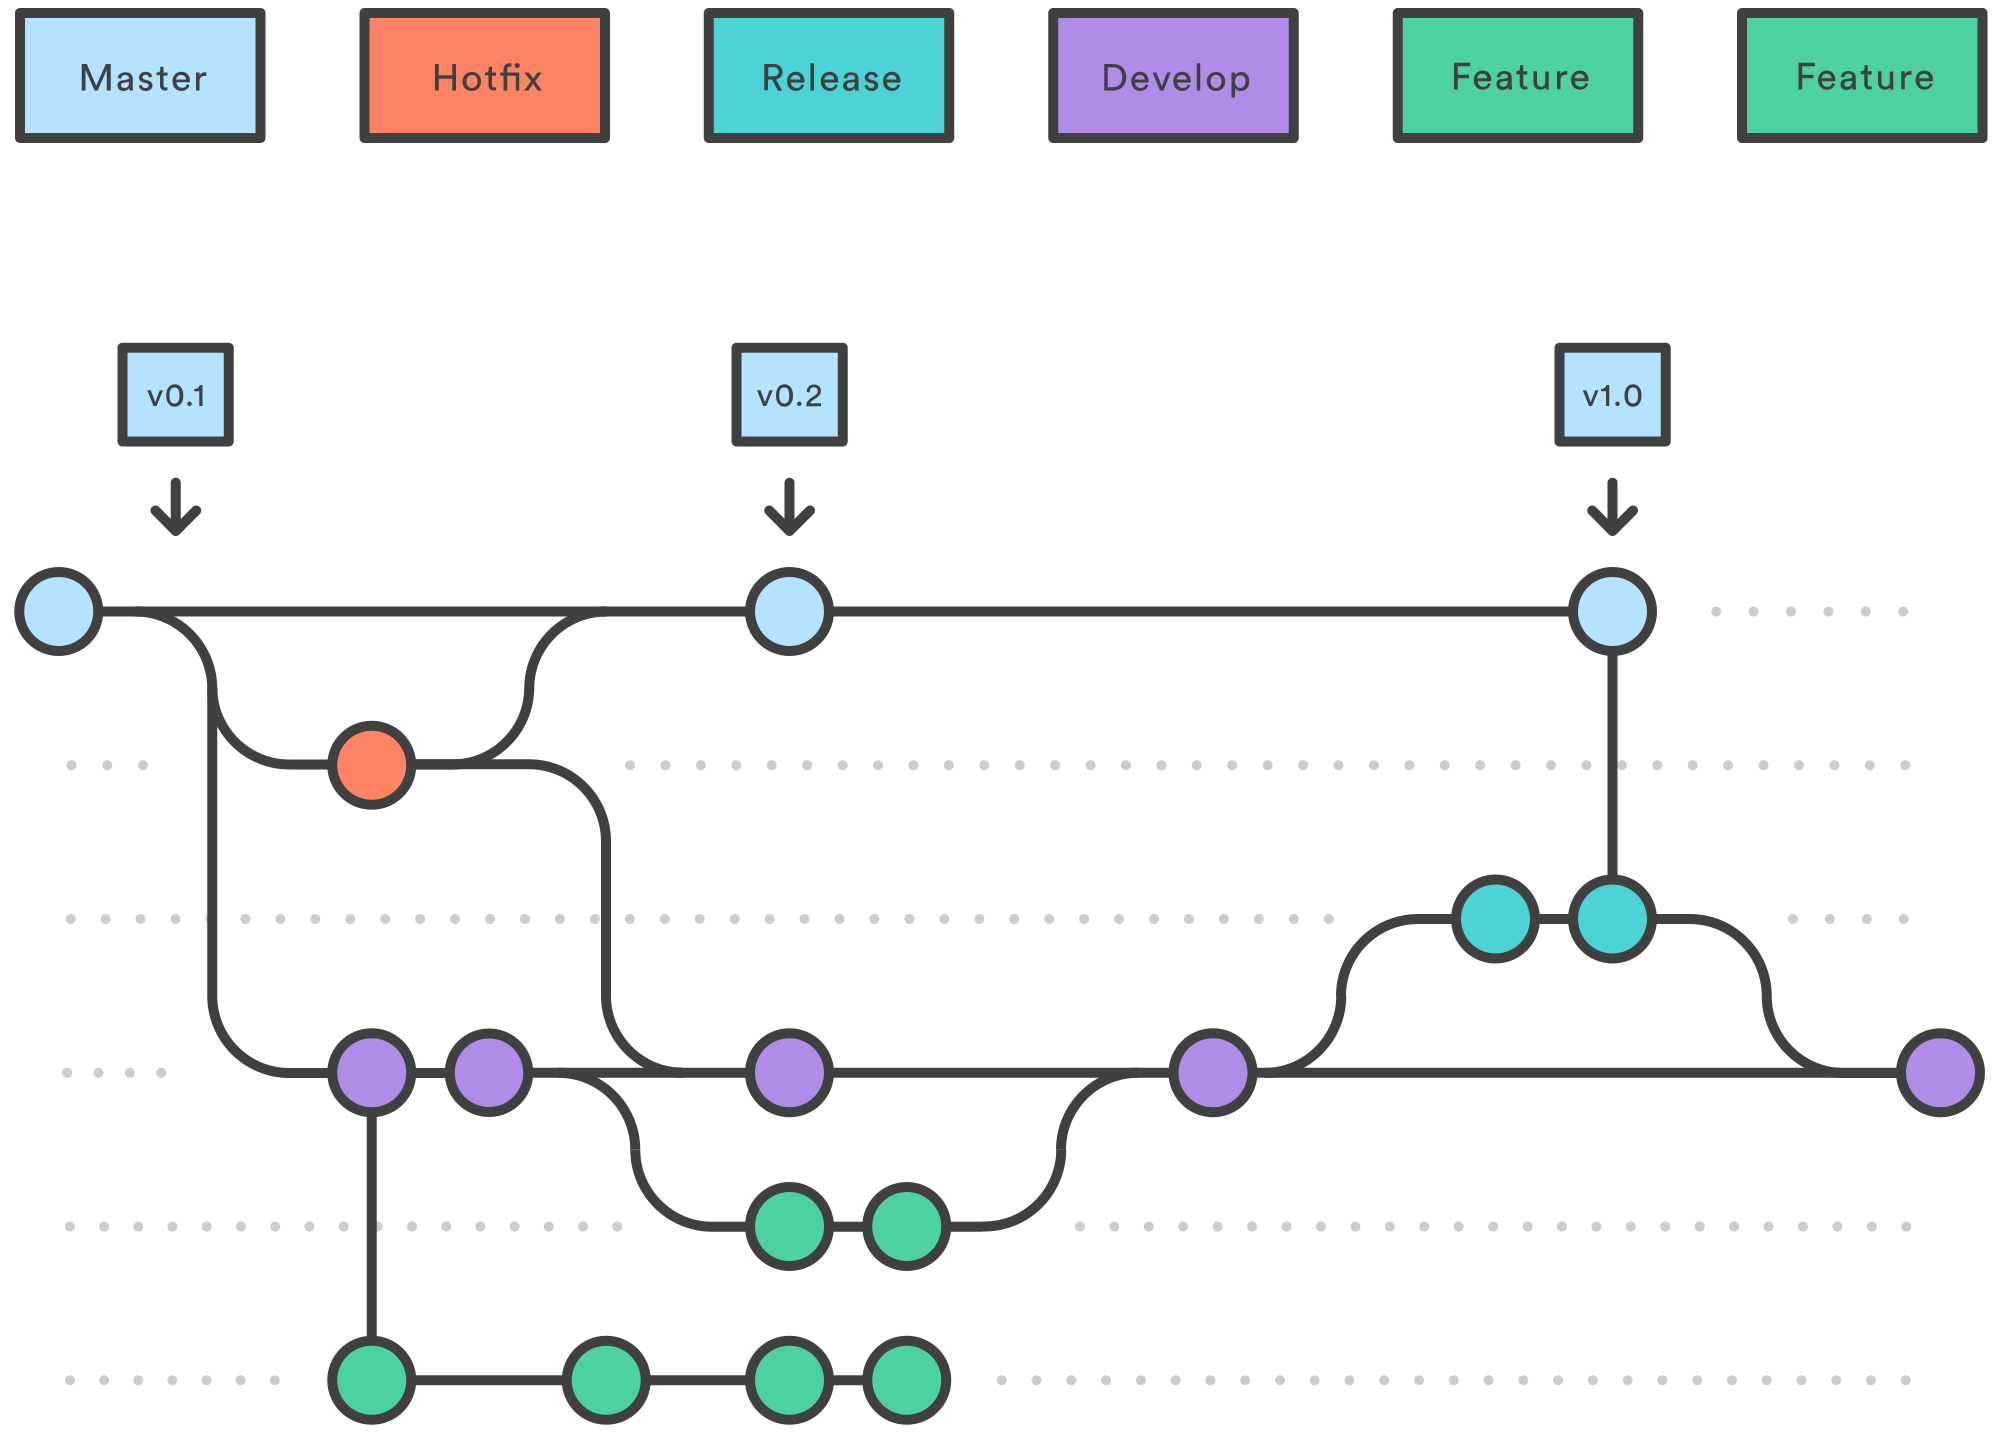
\includegraphics[width=\columnwidth]{img/gitflow}
	\caption[Gitflow]{Gitflow\footnotemark}
\end{figure}
\footnotetext{\cite{atlassian2020}}

Der Gitflow-Workflow definiert ein strenges Branching-Model und gibt jedem Typ von Branch (lediglich differenziert durch ihre Namen) eine spezifische Rolle. \code{Master} wird verwendet, um die Release-History festzuhalten. Hier finden sich Versionen des Projektes, die lauffähig sind und für sich alleine stehen (können). \code{Development} fungiert ähnlich wie \code{Master}, nur enthält es die gesamte Entwicklungshistorie des Projektes. Nun kommen die sogenannten \code{Feature}-Branches ins Spiel. Benannt werden Features hierarchisch. Im Projekt werden folgende zwei Gruppen verwendet: 

\begin{minipage}{\textwidth}
	\texttt{feature/\textbf{backend}/<konkretes-feature>}
	
	\texttt{feature/\textbf{frontend}/<konkretes-feature>}
\end{minipage}

Jedes Feature wird einem Verantwortlichen zugeteilt und wird meist auch von diesem bearbeitet. Sobald ein Feature fertig ist, wird es in \code{Development} zusammengeführt. Somit werden die Abstände zwischen Zusammenführungen verringert und der Arbeitsablauf wird einfacher. Schließlich gibt es auch noch einen Hotfix-Branch für dringende Änderungen.

Im Laufe der Entwicklung haben sich die Vorteile dieser Herangehensweise für das Team deutlich gezeigt. Unterschiedliche Features konnten, nachdem eine grundlegende Programmarchitektur umgesetzt worden ist, meist ohne Probleme zusammengeführt werden. 

\subsection{Jannis Keienburg}

\subsubsection{Latex Sachen}

xxx links as links
Bei der Erstellung der Projekttagebücher ist die Gruppe folgendermaßen vorgegangen: 
Auf der Webseite Tabels Generator (www.tablesgenerator.com) erstellte jedes Teammitglied eine eigene Tabelle, die das individuelle Tagebuch des Mitgliedes bildete. In der Tabelle wurden drei Spalten angegeben: Datum, Dauer und Beschreibung. Der Inhalt der jeweiligen Zeile konnte anschließend eingetragen werde. Das Tagebuch konnte anschließend als. tng Datei heruntergeladen werden oder online gespeichert werden. Aus der erstellten Tabelle wurde anschließend der LaTeX-Code generiert. Auf Authorea (www.authorea.com) wurde anschließend der generierte Code in ein PDF Dokument umgewandelt. 

\begin{figure}[!h]
	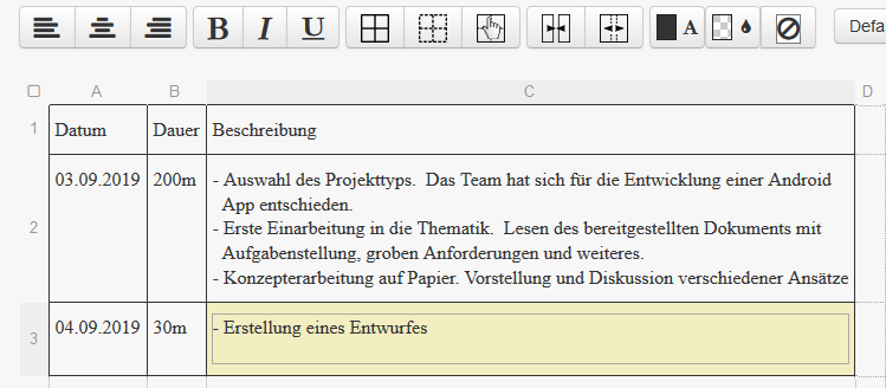
\includegraphics[scale=1]{img/tabels-generator-erstellen}
	\caption[Erstellen einer Tabelle mit Tabels Generator]{Erstellen einer Tabelle mit Tabels Generator\footnotemark}
\end{figure}
\footnotetext{eigene Darstellung}

\begin{figure}[!h]
	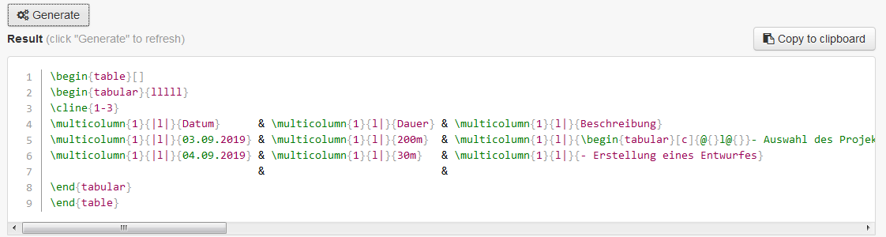
\includegraphics[scale=1]{img/tables-generator-generate}
	\caption[Generierter LaTex Code mit Tabels Generator]{Generierter LaTex Code mit Tabels Generator\footnotemark}
\end{figure}
\footnotetext{eigene Darstellung}

Für die Ausarbeitung wurde ein neues Projekt in Github mit eigenem Repository angelegt. Dort wurden alle Kapitel der Studienarbeit gespeichert. Word diente für Notizen und Entwürfe der Ausarbeitungen, die, in regelmäßigen Abständen, in LaTex umgewandelt wurden. Es wurde Verwendung einer FHDW-Vorlage für LaTex gemacht. Die einzelnen LaTex-Kapitel wurden mit dem Texteditor MikTex erstellt und anschließend in Github hochgeladen. Mit TexStudio wurden anschließend die einzelnen, erstellten Kapitel in ein einziges LaTex-Dokument zusammengeführt.  


\subsection{Khang Pham}

\subsubsection{Erstellung der Funktionalitäten des Mid-Fidelity Prototyps}
\label{subsubsection:erstellung-funktionalitäten-mid-fidelity}

Nach dem der Paper-Prototype erstellt war, wurde das Design des Taschenrechners in PowerPoint finalisiert. Es wurde ein Default-Layout erstellt und die standardmäßige Verteilung der Kacheln des Taschenrechners festgelegt. Dafür wurden in PowerPoint auf einer Folie Form-Objekte angelegt, welche die Kacheln des Taschenrechners darstellen sollten.

\begin{figure}[!h]
	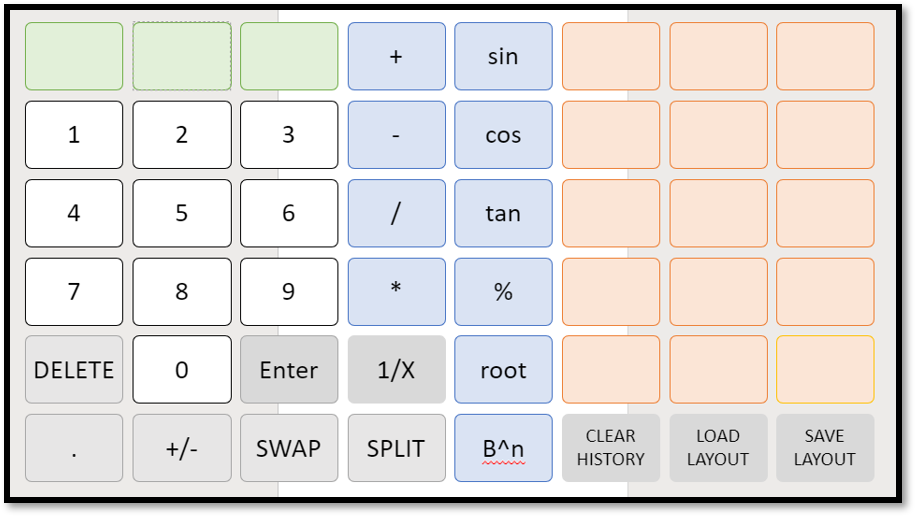
\includegraphics[scale=1]{img/standardlayout-mid-fielty}
	\caption[Standardlayout des Taschenrechners im Mid-Fidelity-Prototyp, aufgebaut aus Form-Objekten]{Standardlayout des Taschenrechners im Mid-Fidelity-Prototyp, aufgebaut aus Form-Objekten\footnotemark}
\end{figure}
\footnotetext{eigene Darstellung}

Um nun Eingaben an dem Prototyp zu ermöglichen, wurden Hyperlinks auf die jeweiligen Form-Objekte gelegt, welche dann auf verschiedene Folien weiterleiteten. Wenn ein Nutzer die PowerPoint-Präsentation startet, kann er nun mit dem Prototypen interagieren. Klickt er beispielsweise auf das Form-Objekt, welches die Zahl ‘‘Eins’‘ darstellt, wird er über den Hyperlink auf eine identische Folie weitergeleitet, in welcher jedoch die ‘‘Eins’‘ im Stack abgebildet ist. Klickt ein Benutzer auf ‘‘AC’‘, wird er auf die erste Folie weitergeleitet, in der der Stack leer ist. Mithilfe der beschriebenen Methode wurden nun die verschiedenen identifizierten Use-Cases nachmodelliert um den Interaktiven Prototypen zu erstellen. Dadurch konnten dann am Prototyp Eingaben getätigt werden, und somit das Konzept der Applikation ausgetestet werden. Beispielsweise das ändern einer Kachel, durch das Gedrückthalten der Taste konnte im Prototyp ausprobiert werden. Auch die Funktionsweise und das Konzept der sogenannten ‘‘History Stacks’‘ (welche näher im Kapitel XXX 7.1.7.1 ‘‘Erstellung des Design Konzeptes des Mid-Fidelity Prototyps’‘ erläutert werden) konnte anhand des interaktiven Prototypens jedem Teammitglied leicht erklärt werden. 


\subsection{Tim Jonas Meinerzhagen}

\subsubsection{Auswahl der Mathebibliothek}

Zur Implementierung der verschiedenen Operanden und ihrer Funktionen haben wir uns dazu entschieden eine Bibliothek zu verwenden. Dies haben wir als sinnvoll erachtet, da zu den geplanten Operanden und Funktionen bereits umfangreiche Implementationen in ausgereiften Bibliotheken verfügbar sind.

Nach einer allgemeinen Recherche über solche Bibliotheken haben wir die beiden Mathebibliotheken Apache Commons Math und JScience genauer betrachtet. 
JScience ist eine der umfangreichsten Java Bibliotheken für wissenschaftliche Anwendungsbereiche und bietet eine Vielzahl Designmodulen für spezielle Anwendungsfälle. Darunter etwa komplexe physikalische Modelle und spezielle Methoden zu beispielsweise Brennwertmethoden oder Modellen der Quantum Physik. Solche wurden allerdings für unsere Applikation nichtbenötigt. Die letzte Aktualisierung der JScience-Bibliothek fand im Jahr 2011 statt. Daraus ist erkenntlich, dass die Bibliothek nicht mehr aktiv weiterentwickelt wird. 

Zum anderen wurde die Bibliothek Apache Commons Math betrachtet. Dieses bietet Vorteile dadurch, dass sie keine externe Abhängigkeit besitzt, abgesehen zu den Commons Komponenten und der Java-Kern-Plattform. Apache Commons Math benötigt lediglich Java 5 oder höher für die 2.0 Version der Mathebibliothek. Ein weiteres Argument für Apache Commons Math ist, dass die Bibliothek auf kleineren, leicht integrierbaren Komponenten aufgebaut ist und keine komplexeren Abhängigkeiten zwischen den einzelnen Komponenten bestehen. Auch eine aufwendige Konfigurierung der Bibliothek ist nicht notwendig. 
Aufgrund der oberen genannten Gründe entschieden wir uns für die Benutzung der Apache Commons Math Bibliothek.


\subsection{Dennis Gentges}

\subsubsection{Blackbox Test – Usability Test}

‘‘Usability beschreibt die Nutzbarkeit eines Produktes oder Dienstes. Gute Usability heißt, dass ein Nutzer schnell und einfach das gewünschte Ergebnis erreicht.’‘ xxx quelle 
Der folgende Usability Test baute dabei auf den zuvor durchgeführten Cognitive Walkthrough von meinem Kollegen Getuart Istogu auf.

Da der Test nur mit wenigen weiteren Benutzern durchgeführt wurde, bot sich ein einfaches Testkonzept an. Basierend auf meiner Erfahrung aus dem Arbeitsumfeld entschied ich mich für das klassische Moderator-Tester Setup. Hierbei gibt es zwei einfache Rollen, den Moderator und die Testperson. Die Testperson soll während des gesamten Testverfahrens ‘‘laut denken’‘. Alle Reaktionen oder Emotionen, wie z.B. Verärgerung, weil eine Funktionalität nicht so funktioniert wie gewünscht, sollen somit dokumentiert und näher beleuchtet werden. Der Moderator wiederum soll den Testteilnehmer nicht beeinflussen, weder durch Gestik/Mimik oder durch Äußerungen. Der Testteilnehmer wird ausschließlich beobachtet und mit offenen Fragen zu weiteren Äußerungen motiviert. 


Bei dem Test merkte der Tester folgende Punkte an:
\begin{itemize}
	\item ‘‘Es wäre schön zwischen normalen Modi für einfache Berechnungen und wissenschaftlichen Modi wechseln zu können.’‘
	\item ‘‘Neben der polnischen Notation sollte auch die normale Notation angeboten werden.’‘ (Dieses Feedback ist jedoch aufgrund der gegebenen Aufgabenstellung zu vernachlässigen).
	\item ‘‘Es ist sehr angenehm bei dem ersten Start der App ein vordefiniertes Layout vorzufinden mit den wichtigsten Funktionen.’‘
\end{itemize}

Das weitere Feedback wurde als zunächst nicht essenziell für die Dokumentation erachtet, wie z.B. die farbliche Gestaltung der App. Dies wäre ausschließlich bei der weiteren Verfolgung und Entwicklung der Applikation in Zukunft hilfreich gewesen, wie z.B. dynamisches Anpassen der Farbe des Layouts oder der Kacheln. 

Zusammenfassend betrachtet war der Tester zufrieden mit der Anwendung, sodass wir uns auf die weitere Umsetzung bzw. Implementierung konzentrieren konnten. 

\subsubsection{Erstellung des Low-Fidelity ''Paper'' Prototyps}
\label{subsubsection:erstellung-low-fidelity-paper}

xxx ganz anz viele quellen
‘‘Paper Prototyping hat sich immer mehr zu einem sehr wichtigen Hilfsmittel im Software Engineering entwickelt.’‘ 

Der Paper Prototype, auch ‘‘Low-Fidelity Prototype” genannt dient in erster Linie im frühen Stadium der Projektenwicklung dazu, ‘‘ein Feed-Back vom Benutzer’‘ einzuholen, ‘‘obwohl noch gar kein Programm geschrieben wurde.’‘  Zum Beginn des Projektes empfiehlt sich Paper Prototyping, da es ‘‘ein sehr preiswertes, schnelles und technisch einfaches Verfahren für einen Usability-Test einer Software’‘  ist.

Um ein gemeinsames Verständnis für einen ersten, einfachen Prototypen im Team zu generieren wurde dieser im Teammeeting angefertigt. Das grundlegende Design wurde schnell gefunden. Den einzelnen Kacheln sollten Klassen zugewiesen werden können (z.B. Funktionen wie AC, Enter oder Delete, Turn Stack) oder aber Zahlenwerte. 

Nachdem der Paper Prototype im Team besprochen wurde und letzte Unstimmigkeiten beseitigt werden konnten, wurde der Prototyp erneut überarbeitet und zusammen mit Herrn Seifert besprochen. Hierbei konnten wir wertvolles Feedback und Verbesserungsvorschläge sammeln, die wir in einer erneuten Überarbeitung des Prototyps umsetzten. 

Als der Paper Prototyp in seiner finalen Fassung von Herrn Seifert abgesegnet wurde, wurde dieser meinem Teamkollegen zur Anfertigung des ‘‘Mid-Fidelity’‘ Prototypen in PowerPoint übergeben.



\subsection{Hendrik Falk}

\subsubsection{Team Koordination}

Ich übernahm als Aufgabe die Koordination des Teams. Dazu zählte die Überwachung des Fortschritts, Kommunikation bei Problemen und die Organisation der Meetings. Ich übernahm die meiste Kommunikation mit dem Auftraggeber Prof. Dr. Thomas Seifert, um Fragen beantwortet zu bekommen, welche während des Projektablaufs auftraten. Um zielführende Kommunikation zu gewährleisten, nahm ich auch an Meetings teil, in denen Inhalte besprochen wurden, zu denen ich keinen direkten Beitrag leisten musste. Ich setzte außerdem ein wöchentliches Meeting auf, in welchem der aktuelle Fortschritt vorgestellt wurde und weiteres Vorgehen sowie Probleme besprochen wurde. Dabei konnte viele Fragen geklärt werden, die dem Projektfortschritt halfen. Den Fortschritt des Projektes und somit auch die fristgerechte Fertigstellung der Applikation und Dokumentation konnte ich mit Hilfe des Meilensteinplans überprüfen, dabei traten keine Probleme auf. 

\begin{tabular}{|c|c|c|c|} 
	\hline
	ID	& Meilenstein &	Soll-Datum & Ist-Datum \\
	\hline	
	1	& Kick-Off Meeting abgehalten & 03.09.2019 & 03.09.2019 \\
	\hline
	2	& Vorgehensmodell ausgewählt & 04.09.2019	& 04.09.2019 \\
	\hline
	3	& Zeitplanung (GANTT) und Kommunikation	& 04.09.2019	& 04.09.2019 \\
	\hline
	4	& Aufgabenverteilung	& 05.09.2019	& 05.09.2019 \\
	\hline
	5	& Mockups fertiggestellt	& 04.01.2019	& 04.01.2020 \\
	\hline
	6	& Android Studio Implementierung	& 25.01.2019	& 25.01.2020 \\
	\hline
	7	& App getestet	& 28.01.2019	& 28.01.2020  \\
	\hline
	8	& Finale App Version	& 04.02.2019	& 04.02.2020 \\
	\hline
	9	& Dokumentation fertig	& 05.02.2019	& 05.02.2020 \\
	\hline
	10	& Abgabe der Ausarbeitung bei Herrn Seifert	& 06.02.2020	& 06.02.2020 \\
	\hline
	11	& Präsentation	& 08.02.2020	& ausstehend \\
	\hline
\end{tabular}
xxx Tabelle beschriftung
Abbildung 28: Soll-Ist-Meilensteinplan


\subsection{Tom Bockhorn}


\subsubsection{Erstellung des Design Konzeptes des Mid-Fidelity Prototyps }
\label{subsubsection:erstellung-des-design-konzeptes-des-mid-fidelity}

Zu Beginn des Projektes wurde zunächst ein Paper-Prototyp mit Hilfe der Anforderungen aus der Aufgabenstellung und in Absprache mit dem Auftraggeber Prof. Dr. Thomas Seifert erstellt. Nachdem das Feedback vom Auftraggeber in der neuesten Version des Paper-Prototyps implementiert wurde, sollte auf Basis des Paper-Prototyps ein Mid-Fidelity-Prototype erstellt werden, das heißt ein interaktiver Prototyp, der das konzipierte Verhalten der Applikation simulieren sollte. Für die Erstellung von Mid-Fidelity-Prototypen gibt es eine große Anzahl an verschiedener Software auf dem Markt. Letzen Endes wurde sich jedoch dafür entschieden Microsoft PowerPoint zu verwenden. Einer der Gründe dafür war, dass PowerPoint Teil des Office Paketes ist, welche den Studierenden von der Fachhochschule zur Verfügung gestellt wird. Somit fielen keine weiteren Kosten für den Erwerb der Software an und es musste auch keine zusätzliche Software heruntergeladen werden. Weiterhin hatten alle Teammitglieder bereits Erfahrung mit PowerPoint gesammelt und mussten dadurch keine Zeit investieren, um den Umgang mit der Software zu erlernen, falls sie den Prototypen verwenden oder anpassen möchten.  

Für die Erstellung des Prototyps wurden auf einer Folie einzelne Form-Objekte angelegt, welche die Knöpfe darstellen sollten. Dadurch konnte eine erste Benutzeroberfläche entworfen werden. In dieser wurde auch das Standardlayout des Taschenrechners (basierend auf dem Paper Prototypen) festgelegt. Wichtig war dabei, dass das Layout an sich nicht fest definiert sein sollte. Ein Nutzer sollte jede Kachel/Taste des Taschenrechners neu belegen können, indem er lange auf einer Kachel gedrückt hält. Das Standardlayout sollte lediglich geladen werden, wenn der Nutzer die App zum ersten Mal startet. Danach sollte der Nutzer das Layout nach Belieben anpassen können und die verschiedenen Layouts abspeichern oder laden zu können.  

\begin{figure}[!h]
	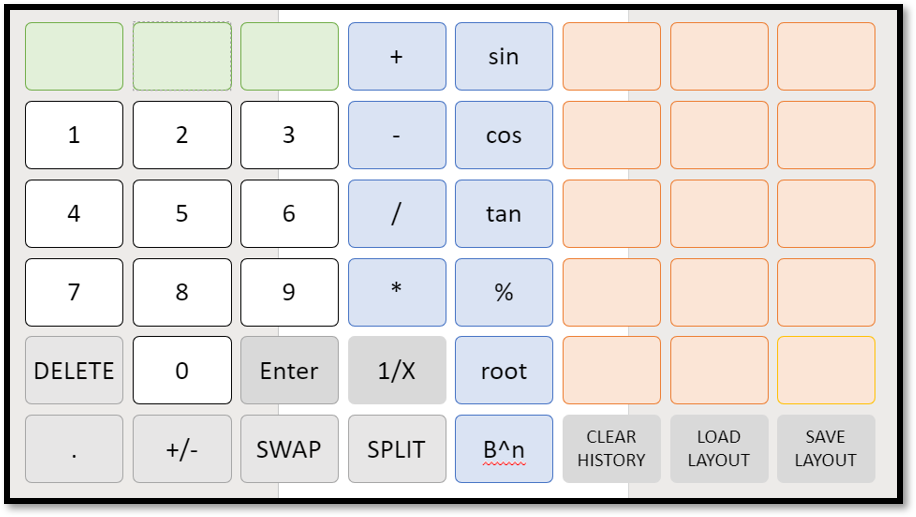
\includegraphics[scale=1]{img/erster-entwurf-mid-fidelty-prototyp}
	\caption[Erster Entwurf des Taschenrechners im Mid-Fidelity-Prototyp]{Erster Entwurf des Taschenrechners im Mid-Fidelity-Prototyp\footnotemark}
\end{figure}
\footnotetext{eigene Darstellung}

Bezüglich der Farbwahl der Kacheln, sollte der Stack des Taschenrechners mit Hilfe grüner Kacheln abgebildet werden, Operanden in weißen Kacheln dargestellt werden, Operatoren in blauen Kacheln und jegliche Einstellungs-Knöpfe (Wie z.B. ‘‘All Clear’‘ oder ‘‘Enter’‘) eine graue Kachelfarbe erhalten. Weiterhin wurde eine weitere Kachelart konzipiert, um der Anforderung einer möglichst geringen Klickzahl für Interaktionen, gerecht zu werden: Der sogenannte ‘‘History Stack’‘ sollte eine orange Kachelfarbe erhalten. Das Konzept des History Stacks ist, dass jegliche Zwischenergebnisse in diesem gespeichert werden, so dass ein Benutzer bereits einmal verwendete Zahlen nicht erneut eintippen muss, auch wenn diese bereits aus dem Stack verschwunden sind. Das Besondere an dem History Stack ist dabei, dass nicht nur Zwischenergebnisse, sondern auch alle Eingabewerte wie Zahlen, Gleichungen oder Matrizen in diesem gespeichert werden. Beispielsweise wenn ein Nutzer die Zahl ‘‘25,5’‘ eintippt wird diese in dem normalen Stack gespeichert, gleichzeitig erscheint die 25,5 aber auch im History Stack (vorausgesetzt die Taste 25,5 existiert zu diesem Zeitpunkt noch nicht). Addiert der Nutzer nun fünf, verschwindet die 25,5 aus dem normalen Stack, da dort nun das Ergebnis 30,5 angezeigt wird. Im History Stack ist die 25,5 jedoch immer noch vorhanden, so dass der Nutzer, sollte er die 25,5 nochmals verwenden wollen, jederzeit über einen einzelnen Tastendruck 25,5 in den normalen Stack ablegen kann. Darüber hinaus wurde noch ein Standardlayout für den „Porträtmodus“ des Tabletts entwickelt. Bei einer vertikalen Ausrichtung sollte automatisch dieses Design geladen werden. 

Es wurde sich dazu entschieden, dass die Anzahl an Kacheln im vertikalen Modus für eine verbesserte Übersichtlichkeit verringert werden sollte. Die Kachelfarben sollten jedoch identisch bleiben um den Wiedererkennungswert der Kacheln zu erhöhen und somit für eine verbesserte Usability zu sorgen.

\subsection{Getuart Istogu}

\subsubsection{Benutzerfreundlichkeit – Cognitive Walkthrough}
Neben dem Projektmanagement und der eigentlichen Programmierung musste ebenfalls gewährleistet können, dass der Benutzer intuitiv mit der Anwendung umgehen kann. Dazu untersuchte ich folgende Fragestellungen:

\begin{itemize}
	\item 1. Wie kann der Benutzer komfortabel die Kacheln spezifizieren, die die Operanden beinhalten? Wie kann er diese ändern? Wie kann er die Reihenfolge der Operanden spezifizieren?
	\item 2. Wie kann der Benutzer komfortabel die Kachel oder die Kacheln spezifizieren, in der das Ergebnis bzw. die Ergebnisse einer Operation gespeichert wird/werden?
\end{itemize}
xxx zu 1 / 2

Generell soll sich die App durch eine hohe Benutzerfreundlichkeit auszeichnen, die einfach, intuitiv und einheitlich bedienbar ist, aber auch zeitgleich eine minimale Menge von Interaktionen für die gewünschten Funktionalitäten erfordert.

Dazu startete ich mit einem Cognitive Walkthrough des Mid-Fidelity Prototyps und überlegte mir, welche Anforderungen ich als Benutzer stellen würde. 

Ein Cognitive Walkthrough ist eine Experten-basierte Methode der Usability Inspektion. Bei der Durchführung eines Cognitive Walkthroughs simuliert ein Usability Engineer Benutzerkognitionen bei der zielorientierten Nutzung eines interaktiven Systems […].  xxx quelle

Nach weiteren Verbesserungen wurde dieser Herrn Seifert vorgelegt, wodurch weitere Verbesserungsvorschläge gesammelt und der Prototyp angepasst werden konnte. 
Als die wichtigsten Design- und Funktionalitätsanforderungen kristallisierten sich dabei durch den Cognitive Walkthrough, Tests und Materialanalyse folgende Anforderungen heraus:
\begin{itemize}
	\item Die App soll sowohl horizontal als auch vertikal benutzbar sein.
	\item Die Kacheln sollen dynamisch anpassbar sein: Durch ‘‘halten’‘ auf einer Kachel mit dem Finger soll der Typ dieser angepasst werden können.
	\item Beim ersten Start der App soll ein Standartlayout geladen werden, um die Navigation am Anfang zu erleichtern.
	\item Gängige Bezeichnungen (wie von normalen Taschenrechnern bekannt) sollen beibehalten werden.
	\item Beim Neustarten der App soll das zuletzt bekannte Layout wieder geladen werden.
\end{itemize}

Diese Anforderungen wurden im Team kommuniziert und im Mid-Fidelity Prototyp sowie in der Implementierung nach Android Studio berücksichtigt. Im Anschluss sollte ein Usability Test als Blackbox Test mit einem Anwender Aufschlüsse darüber geben, ob die angedachte bisherige Umsetzung zufriedenstellend ist.

